\documentclass[
]{beamer}

\usepackage[english]{babel}
\usepackage[utf8]{inputenc}
\usepackage[T1]{fontenc}
\usepackage{lmodern}
\usepackage{csquotes}
\usepackage{expl3,biblatex}
\addbibresource{sources.bib}
\usepackage{booktabs}
\usetheme[
  workplace=fi,
  fonts=none,
]{MU}
\usepackage{textalpha}
\usepackage{subfigure}
\usepackage{wrapfig}
\usepackage{tikz}
\usepackage{appendixnumberbeamer}

\title[Visualisation and Annotation of VolSeg Data in Mol*]{Lightweight Visualisation and Annotation of Volumetric and Segmentation Data in Mol*}
\subtitle[Master's Thesis Defense]{Master's Thesis Defense}
\author[D. Tichý]{Author:\hspace{0.63em}Bc. Dominik Tichý\texorpdfstring{\\}{, }Advisor: RNDr. Tomáš Raček, Ph.D.}
\institute[FI MU]{Faculty of Informatics, Masaryk University}
\date{January 30, 2026}
\subject{Presentation Subject}
\keywords{Mol*, Mol* VS, MolViewSpec, MolViewStories, volumetric data, segmentations, visualization, bioinformatics}

\begin{document}

\begin{frame}[plain,noframenumbering]
\maketitle
\end{frame}

\begin{frame}{Motivation}
  \begin{itemize}
    \item Rapid growth of microscopy data (e.g., Cryo-EM, Cryo-ET) \footfullcite{kuhlbrandt2014resolution}
    \item Critical in structural biology and drug design (e.g., SARS-CoV-2 spike protein characterization) \footfullcite {wrapp2020covid}
    \item Need for a web-based tool to visualize and annotate
  \end{itemize}
\end{frame}

\begin{frame}{Technologies}
  \begin{itemize}
    \item Mol* platform
    \item Mol* Volumes and Segmentation (Mol* VS) \footfullcite{Chareshneu2024Volseg}
    \begin{itemize}
      \item Difficult to use and maintain
      \item Lacks interoperability
      \item Siloed data formats
    \end{itemize}
    \item MolViewSpec (MVS) \footfullcite{Midlik2025MolViewSpec}
    \begin{itemize}
      \item Declarative standard
      \item Describes ``what'' the scene looks like, not ``how'' to build it
    \end{itemize}
    \item MolViewStories
    \begin{itemize}
      \item UI builder for MolViewSpec
    \end{itemize}
  \end{itemize}
\end{frame}

\begin{frame}{Mol* VS Architecture}
  \begin{figure}
    \includegraphics[width=1\textwidth,height=0.8\textheight,keepaspectratio]{./images/volseg-arch.pdf}
    % \caption{Mol* VS Architecture}
  \end{figure}
\end{frame}


\begin{frame}{Goals}
  \begin{itemize}
    \item Move the legacy Mol* VS client to MolViewSpec
    \item \textbf{Contribution 1:} Create a conversion library
    \item \textbf{Contribution 2:} Web application for non-technical users
  \end{itemize}
\end{frame}

\begin{frame}{Data Mapping}
  \begin{itemize}
    \item \textbf{Volumes}
    \begin{itemize}
      \item 3D scalar grids representing electron density or potential
      \item Isosurface, grid slice
    \end{itemize}
    \item \textbf{Segmentations}
    \begin{itemize}
      \item Convert intensity signals into discrete objects
      \item Lattices, meshes, geometric primitives
    \end{itemize}
    \item \textbf{Annotations}
    \begin{itemize}
      \item Define semantic meaning and visual styling
      \item Examples include color, opacity, and labels
    \end{itemize}
  \end{itemize}
\end{frame}

\begin{frame}{Data Mapping}
  \begin{figure}
    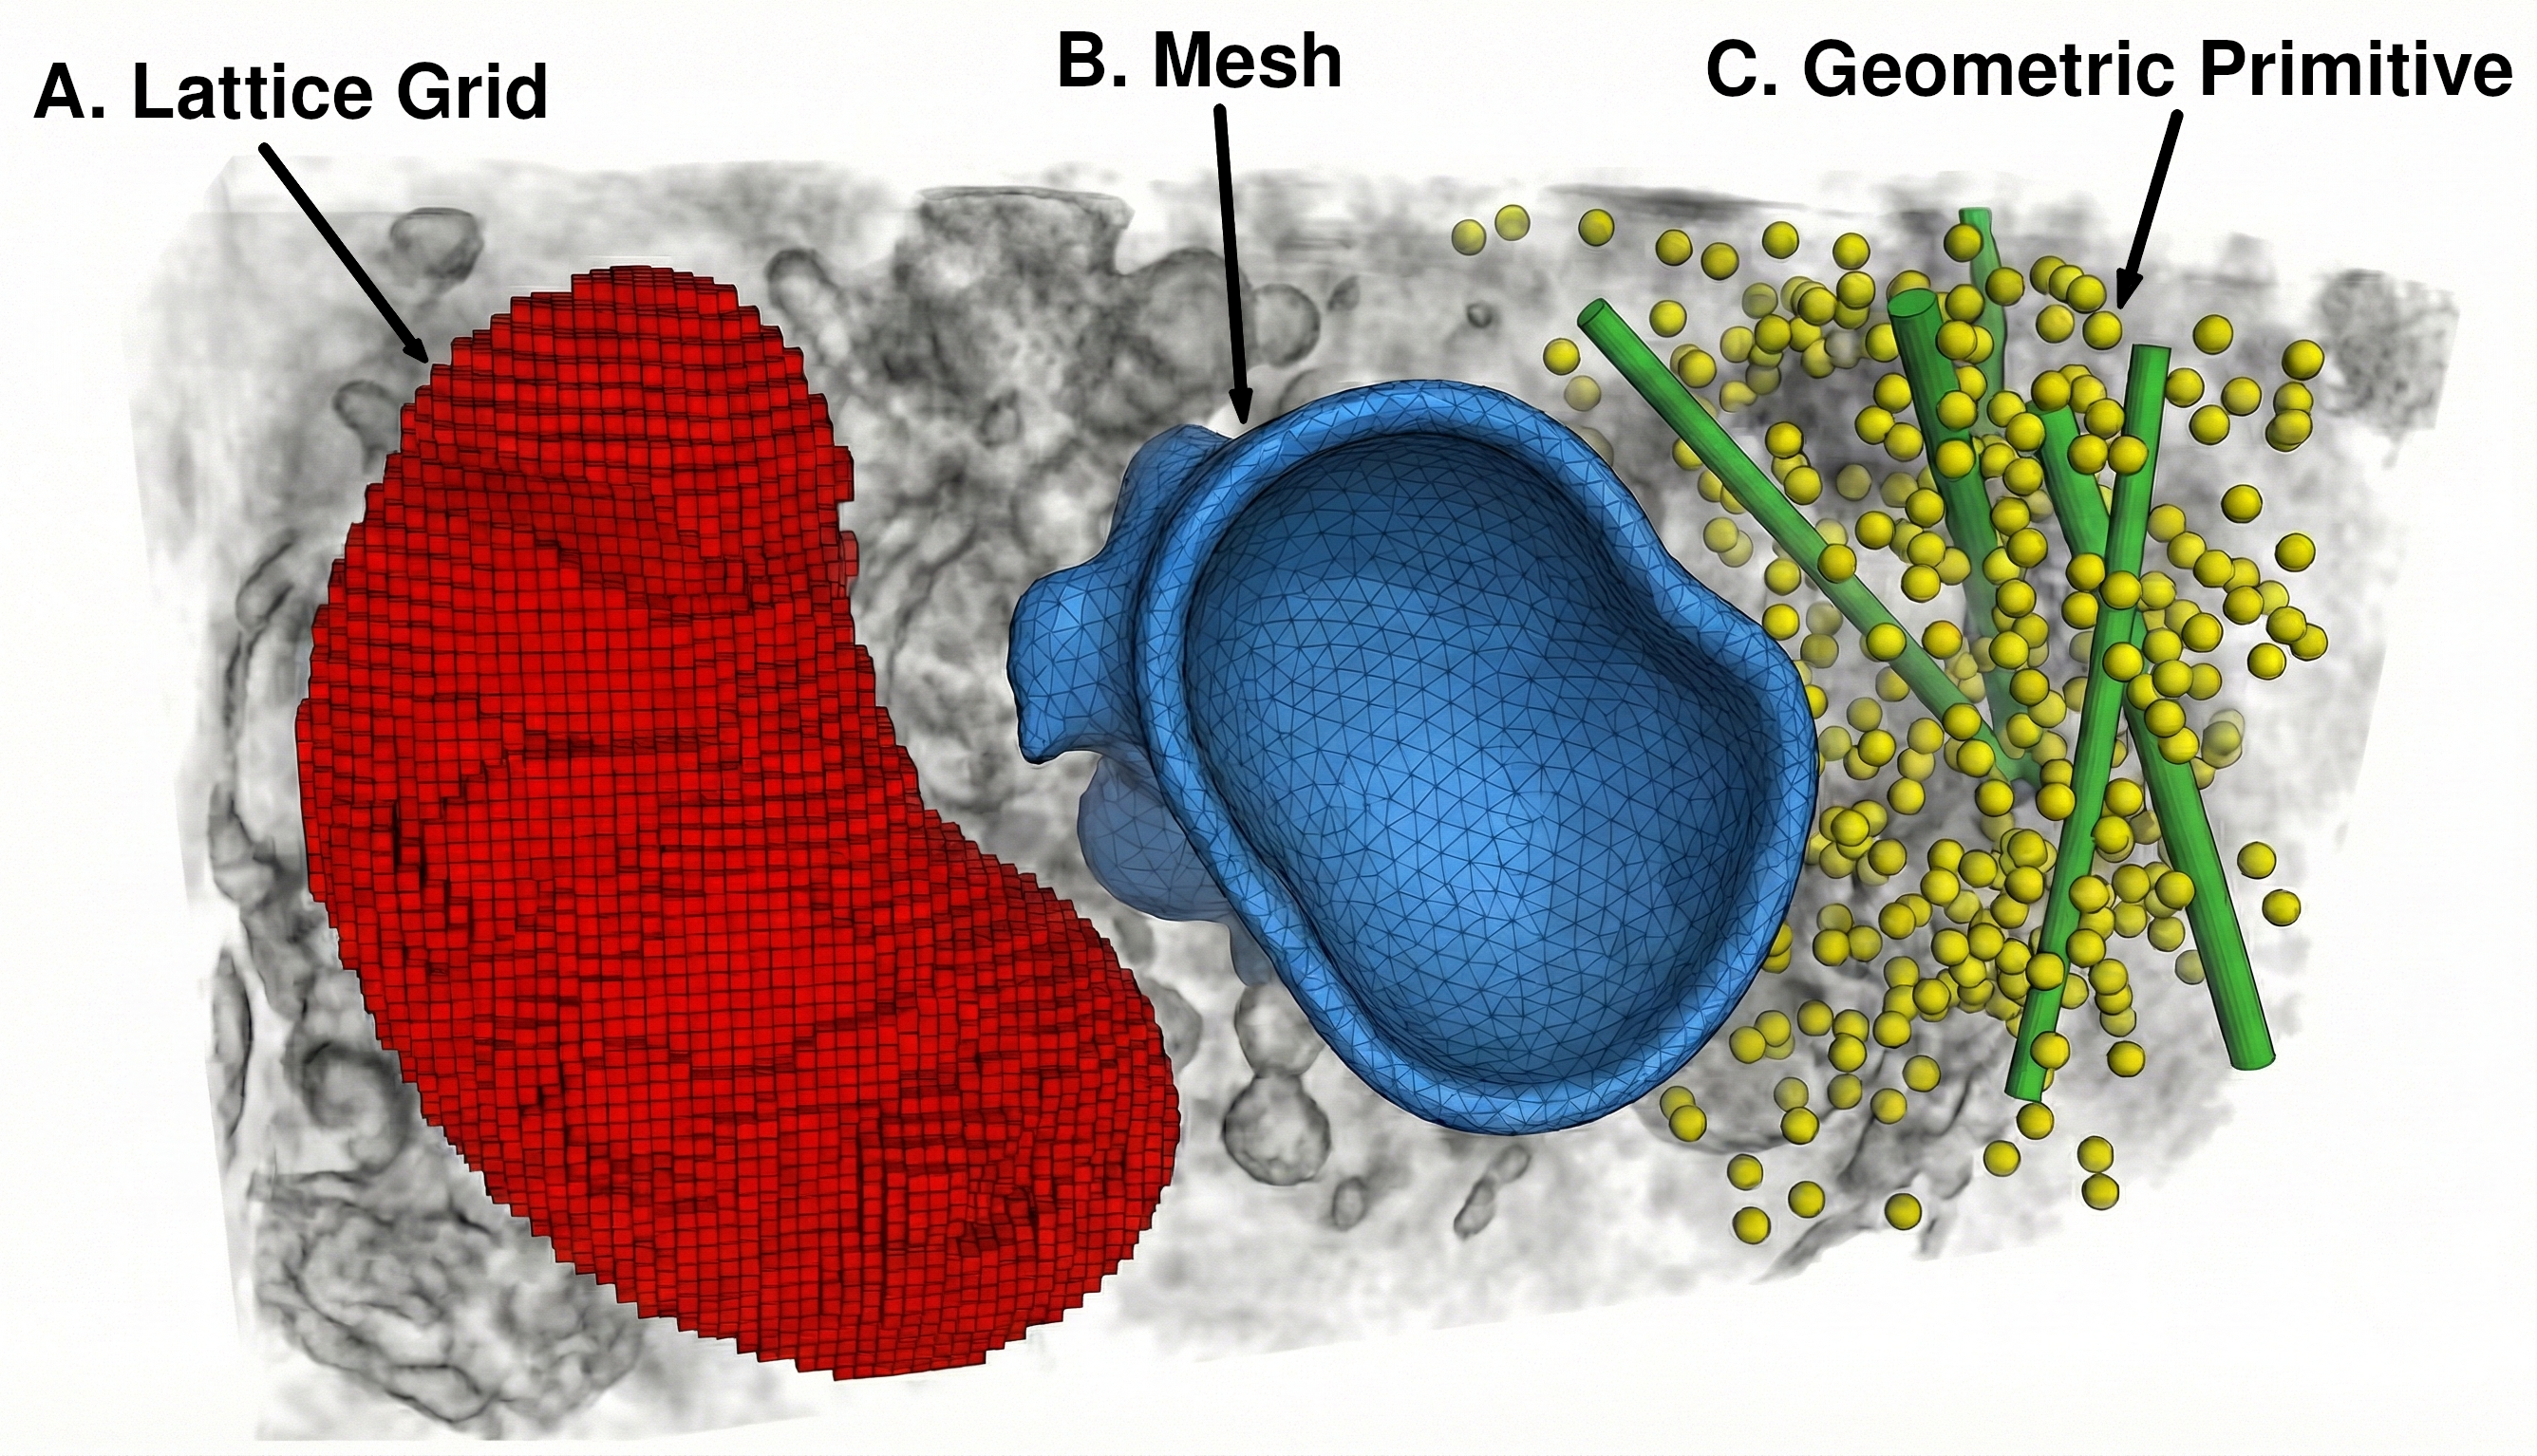
\includegraphics[width=1\textwidth,keepaspectratio]{./images/segmentation-comparison.png}
    % \caption{Segmentation types.}
  \end{figure}
\end{frame}

\begin{frame}{Volumetric Data}
  \begin{figure}
    \centering
    \includegraphics[height=0.8\textheight,keepaspectratio]{./images/volume-mapping-crop.pdf}
    % \caption{Mapping CVSX to MVSX}
  \end{figure}
\end{frame}

\begin{frame}{Lattice Segmentation}
  \begin{figure}
    \centering
    \includegraphics[height=0.85\textheight,keepaspectratio]{./images/lattice-mapping-crop.pdf}
    % \caption{Mapping CVSX to MVSX}
  \end{figure}
\end{frame}

\begin{frame}{Mesh \& Geometric Segmentation}
  \begin{figure}
    \centering
    \includegraphics[height=0.9\textheight,keepaspectratio]{./images/segm-mapping-crop.pdf}
    % \caption{Mapping CVSX to MVSX}
  \end{figure}
\end{frame}


\begin{frame}{Conversion Library --- Architecture}
  \textbf{``ETL'' Architecture:}
  \begin{itemize}
    \item \textbf{Extract:} Validate and parse CVSX
    \item \textbf{Transform:} Convert to intermediate representation
    \item \textbf{Load:} Serialize to MVSX or MVStory format
  \end{itemize}
  \begin{figure}
    \includegraphics[width=0.9\textwidth,keepaspectratio]{./images/etl-overview-crop.pdf}
    % \caption{Mapping CVSX to MVSX}
  \end{figure}
\end{frame}

\begin{frame}{Conversion Library --- Extract}
  \begin{figure}
    \centering
    \subfigure{\includegraphics[width=0.25\textwidth,keepaspectratio]{images/extraction-crop.pdf}}
    \hspace{1cm}
    \subfigure{\includegraphics[width=0.45\textwidth,keepaspectratio]{images/cvsx_entry-crop.pdf}}
    % \caption[Extraction]{Extraction of CVSX data.}
  \end{figure}  
\end{frame}

\begin{frame}{Conversion Library --- Transform \& Load}
  \begin{figure}
    \centering
    \subfigure{\includegraphics[width=0.25\textwidth,keepaspectratio]{images/transform-crop.pdf}}
    \hspace{1cm}
    \subfigure{\includegraphics[width=0.45\textwidth,keepaspectratio]{images/transform-load.pdf}}
    % \caption[Extraction]{Extraction of CVSX data.}
  \end{figure}  
\end{frame}

\begin{frame}{Conversion Library --- Results}
  \textbf{Visual Fidelity:}
  \begin{itemize}
    \item Verified on 14 diverse datasets from EMDB, IDR, EMPIAR
  \end{itemize}

  \textbf{File Size:}
  \begin{itemize}
    \item Minimal overhead ($<5\%$) for most mappings
    \item Except for lattice-to-mesh conversion ($10-50\%$)
  \end{itemize}
  
  \textbf{Improvements:}
  \begin{itemize}
    \item Fixed missing volumes, restored color annotations
    \item Corrected author-defined contour levels
    \item Proper isosurface capping (watertight meshes)
    \item Batched geometric primitives (performance improvement)
  \end{itemize}
\end{frame}

\begin{frame}{Conversion Library --- Improvements}
  \begin{figure}
    \centering
    \subfigure[CVSX]{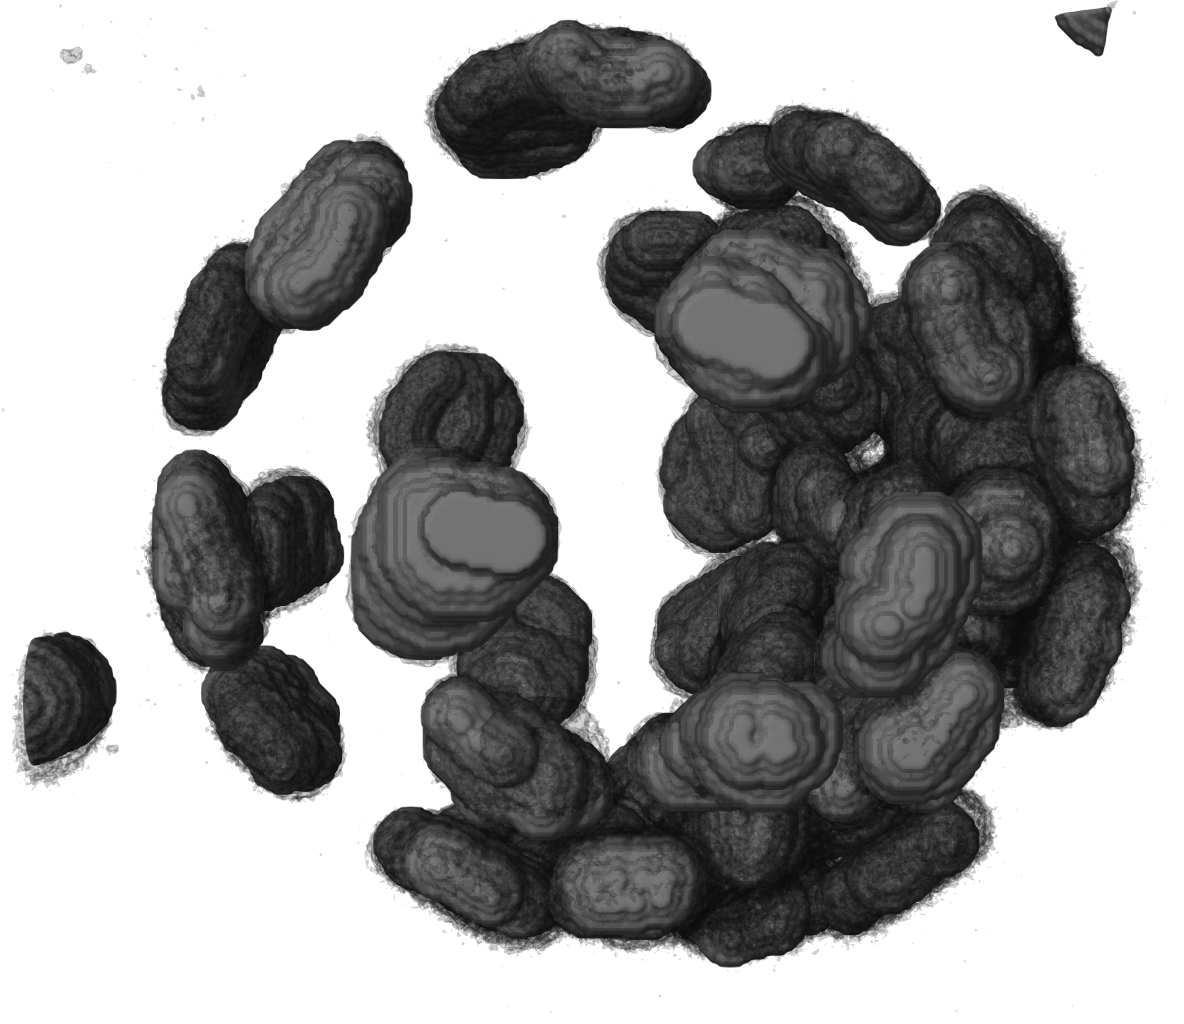
\includegraphics[width=0.4\textwidth]{images/idr-6001240-cvsx.png}}
    \subfigure[MVSX]{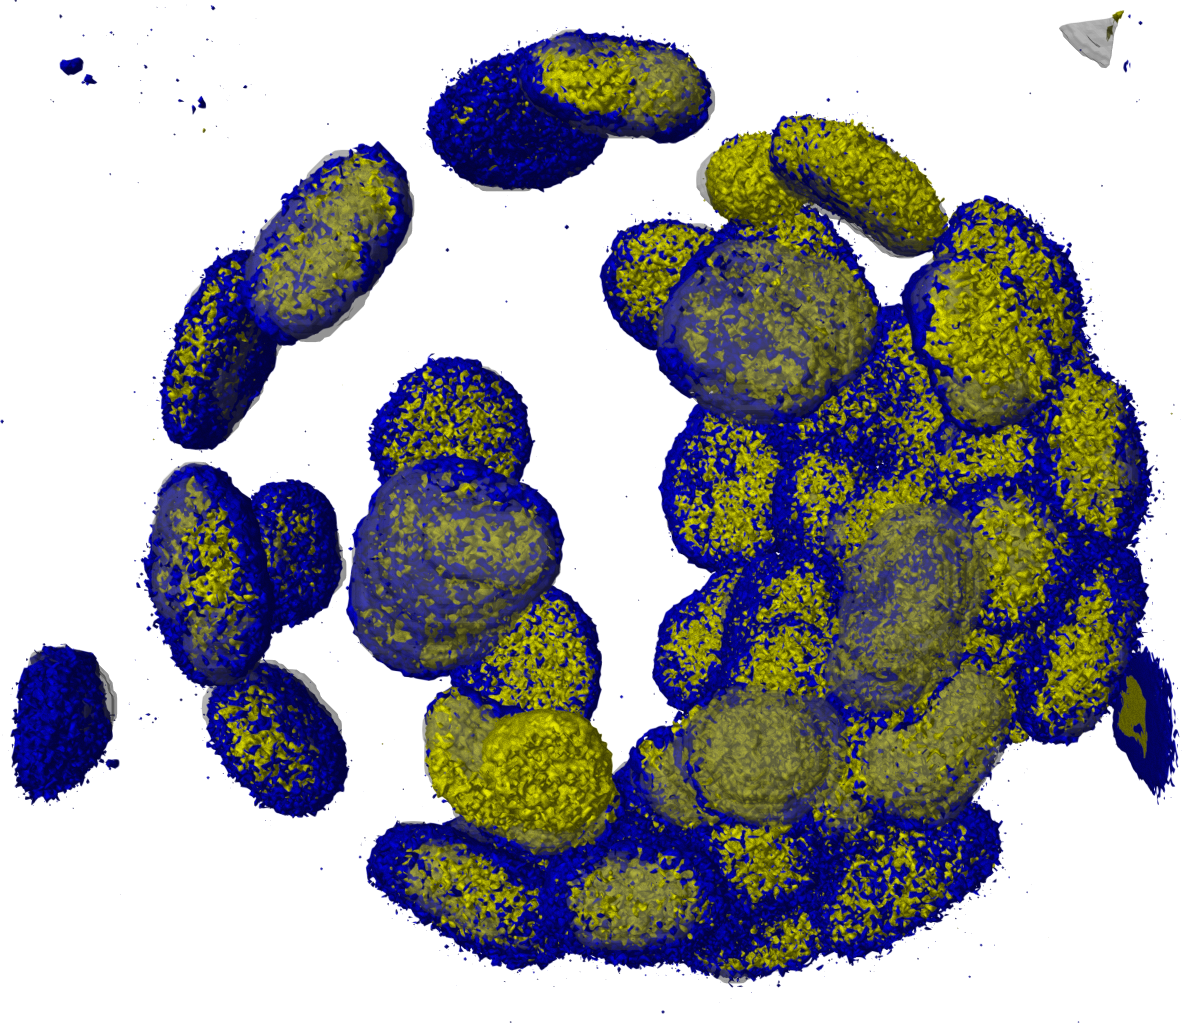
\includegraphics[width=0.4\textwidth]{images/idr-6001240-mvsx.png}}
    \caption[Correction of missing color annotations]{Correction of missing color annotations.}
  \end{figure}  
\end{frame}

\begin{frame}{Conversion Library --- Improvements}
  \begin{figure}
    \centering
    \subfigure[CVSX]{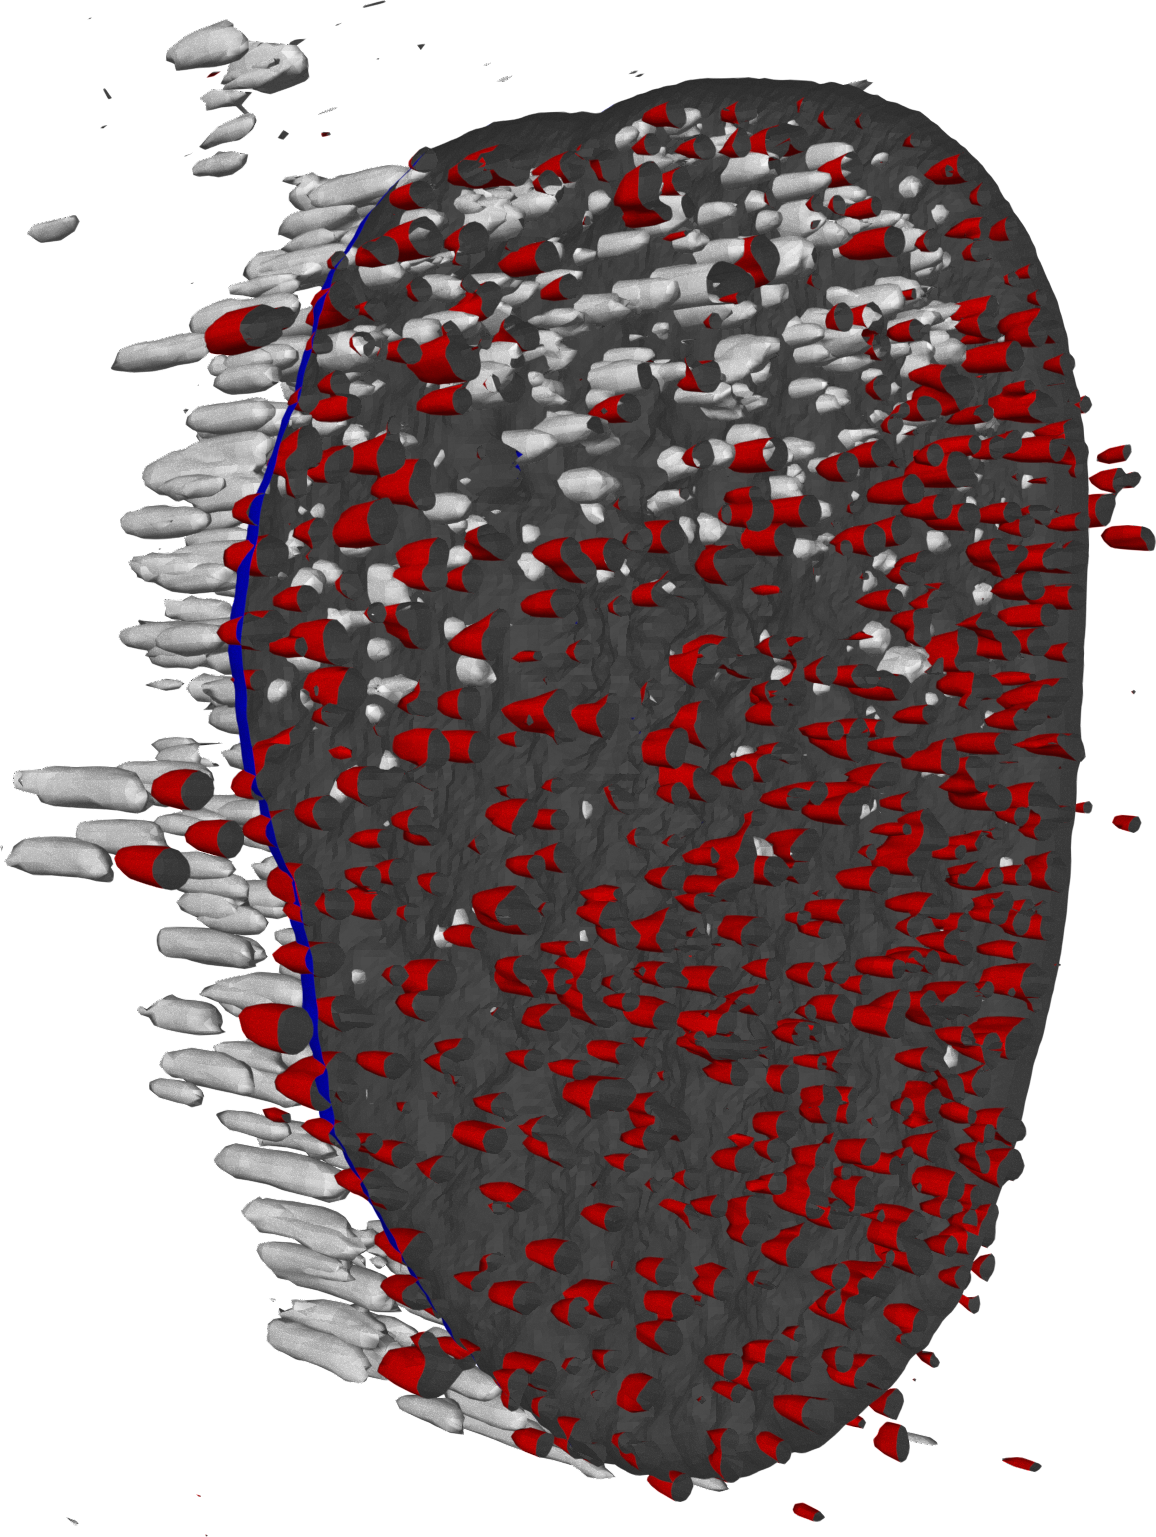
\includegraphics[width=0.3\textwidth]{images/missing-face-cvsx.png}}
    \subfigure[MVSX]{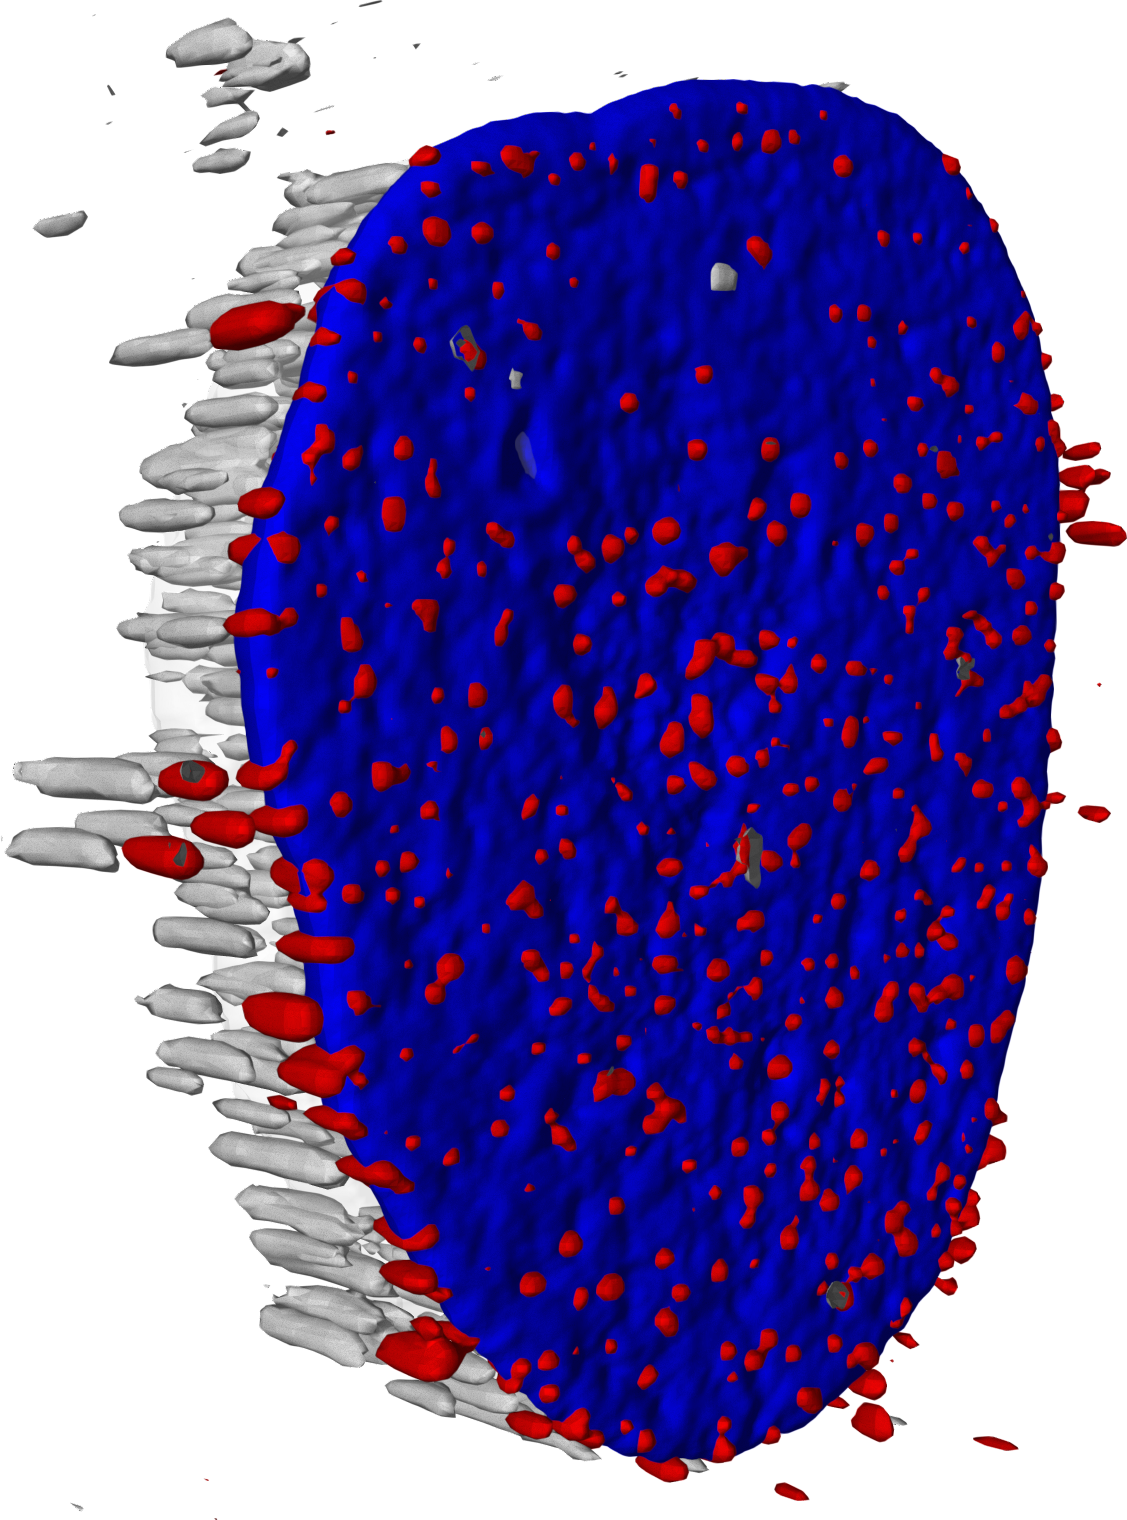
\includegraphics[width=0.3\textwidth]{images/missing-face-mvsx.png}}
    \caption[Correction of isosurface capping]{Correction of isosurface capping.}
  \end{figure}  
\end{frame}

\begin{frame}{Conversion Library --- Improvements}
  \begin{figure}
    \centering
    \subfigure[CVSX]{
\includegraphics[width=0.3\textwidth]{images/contour-missing.png}}
    \subfigure[MVSX]{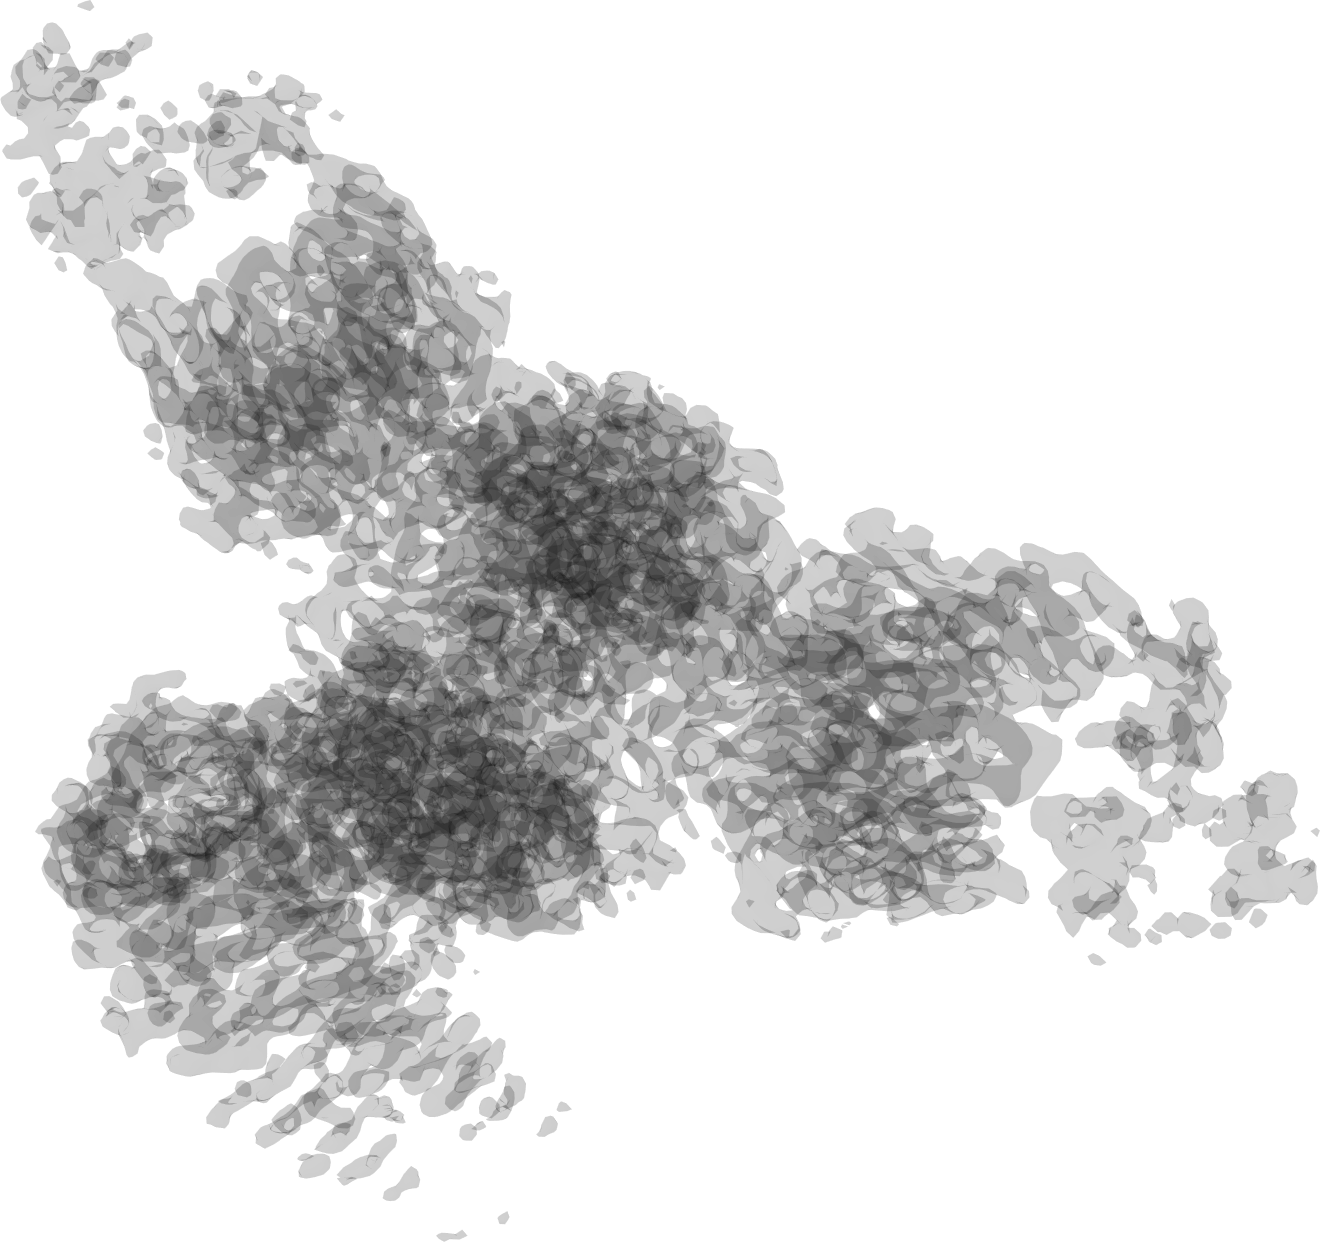
\includegraphics[width=0.3\textwidth]{images/contour-present.png}}
    \caption[Correction of missing author-defined contour levels]{Correction of missing author-defined contour levels.}
  \end{figure}  
\end{frame}

\begin{frame}{Web Application}
  \begin{itemize}
    \item The library is a CLI tool; biologists need a GUI
    \item \textbf{Dashboard}: Manage entries and storage quotas
    \item \textbf{WYSIWYG Editor}: Interactively update colors, opacities, and isovalues
    \item \textbf{Sharing}: Persistent URLs and export to MolViewStories
  \end{itemize}
\end{frame}

\begin{frame}{Web Application --- Architecture}
  \textbf{Main Components:}
  \begin{itemize}
    \item \textbf{Frontend:} React SPA
    \item \textbf{Backend:} FastAPI
    \item \textbf{Storage:} PostgreSQL + MinIO
    \item \textbf{Auth:} EINFRA AAI
  \end{itemize}
\end{frame}

\begin{frame}{Web Application --- Deployment}
  \textbf{Infrastructure:}
  \begin{itemize}
    \item Containerized with Docker
    \item Deployed on CERIT-SC Kubernetes cluster
    \item Helm charts for configuration management
    \item CI/CD pipeline via GitHub Actions
  \end{itemize}

  \textbf{Available at:}
  \begin{itemize}
    \item \small{\url{https://web.volseg-editor.dyn.cloud.e-infra.cz/}}
    \item \small{\url{https://api.volseg-editor.dyn.cloud.e-infra.cz/}}
  \end{itemize}
\end{frame}

\begin{frame}{Web Application --- Results}
  \begin{figure}
    \includegraphics[width=1\textwidth,keepaspectratio]{./images/dashboard2.png}
    \caption{User's dashboard in the web application.}
  \end{figure}
\end{frame}

\begin{frame}{Web Application --- Results}
  \begin{figure}
    \includegraphics[width=1\textwidth,keepaspectratio]{./images/viewer2.png}
    \caption{Annotations editor in the web application.}
  \end{figure}
\end{frame}


\begin{frame}{Conclusion}
  \begin{itemize}
    \item Replaced the Mol* VS client with MolViewSpec
    \item Conversion library for data migration
    \item Provide access to non-programmers
    \item Contributed to a paper \cite{Chareshneu2024Volseg}
  \end{itemize}
\end{frame}

\section{\bibname}
\begin{frame}[t, allowframebreaks]{\bibname}
\printbibliography[heading=none]
\end{frame}

\newenvironment{outroframe}{
  \begingroup
  \setbeamercolor{background canvas}{bg=mubeamer@label}
  \setbeamercolor{normal text}{fg=black}
  \usebeamercolor[fg]{normal text}
  \begin{frame}[plain, noframenumbering, environment=outroframe]
  \vfill
  \centering
}{
  \vfill
  \end{frame}
  \endgroup
}
\begin{outroframe}
    \Huge \textbf{Thank You for Your Attention}
\end{outroframe}

\appendix

\section{Otázky oponenta}

\subsection[Otázka 1]{Otázka 1}

\begin{frame}
  \begin{block}{Otázka oponenta 1}
    Narazil jste na nějakou vlastnost nebo typ dat z formátu CVSX, kterou nebylo možno převést do nových formátů MVSX a MVStory?
  \end{block}
  \begin{itemize}
    \item Ano, uživatelské rozhraní pro Mol* VS klienta a CVSX metadata (např. dimenzionalita volumetrických dat)
    \item Uživatelské rozhraní lze nahradit novým rozšířením Mol* za pomocí metadat v MVS souboru
    \item MVS metadata lze využít i pro CVSX metadata
  \end{itemize}
\end{frame}

\subsection[Otázka 2]{Otázka 2}

\begin{frame}
  \begin{block}{Otázka oponenta 2}
    Je nějaký limit velikosti dat, nad který není vaše webová aplikace schopna data zobrazit?
  \end{block}
  \begin{itemize}
    \item Ano, velikost dat je omezena možnostmi Mol* Vieweru
    \item Závisí na velikosti RAM stroje a nastavení limitů pro paměť v prohlížeči
  \end{itemize}
\end{frame}

\subsection[Otázka 3]{Otázka 3}

\begin{frame}
  \begin{block}{Otázka oponenta 3}
    Jak by bylo možno odstranit drobné vizuální odchylky v renderování, které zmiňujete v sekci 3.4.4?
  \end{block}
  \begin{itemize}
    \item answer
  \end{itemize}
\end{frame}

\makeoutro
\addtocounter{framenumber}{-1}

\end{document}
